\documentclass[conference,letterpaper]{IEEEtran}
\IEEEoverridecommandlockouts

%
% ─── PREAMBLE ───────────────────────────────────────────────────────────────────
% \usepackage[a4paper, total={7in, 8in}]{geometry}
% \usepackage{fancyhdr}

% \fancypagestyle{plain}{%
%    \fancyhf{}
%    \fancyfoot[C]{\iffloatpage{}{\thepage}}
%    \renewcommand{\headrulewidth}{0pt}}
% \pagestyle{plain}

\usepackage[T1]{fontenc} % Use 8-bit encoding that has 256 glyphs
\usepackage{fourier} % Use the Adobe Utopia font for the document - comment this line to return to the LaTeX default
\usepackage[english]{babel} % English language/hyphenation
\usepackage{amsmath,amsfonts,amsthm} % Math packages
\usepackage{bm}
\usepackage{graphicx}
\usepackage{mathrsfs}
\usepackage{apacite}
\usepackage{float}
\usepackage{listings}
\usepackage{color}
\usepackage{enumitem}
\usepackage{pgfplots}
\usepackage{tabularx}

\usepackage{mathtools}  
\mathtoolsset{showonlyrefs}  

\lstset{
    basicstyle=\footnotesize,
    columns=fullflexible,
    breaklines=true,
    tabsize=2,
    postbreak=\mbox{\textcolor{red}{$\hookrightarrow$}\space}
}

\graphicspath{{./images/}}

%
% ──────────────────────────────────────────────────────────────────── II ──────────
%   :::::: R E P O R T   O P E N I N G : :  :   :    :     :        :          :
% ──────────────────────────────────────────────────────────────────────────────
%
% \title{Advanced Algorithms Assignment 2}
% \author{Zaymon Foulds-Cook}

\begin{document}

\title{Cross Entropy Method and BFGS for Optimization of 2-Dimensional Bonded-Molecule Clusters}
\author{\IEEEauthorblockN{Zaymon Foulds-Cook s5017391}
\IEEEauthorblockA{Griffith University School of Information Communication Technology}}

\maketitle

\begin{abstract}
    This paper defines a real coded implementation of the Cross Entropy Optimization Method as both a local and global optimizer in order to find optimal low energy configurations of bonded 2-dimensional molecules. The algorithm was able to find optimum and near optimum values for molecules of up to length 20 and found configurations within 5-15\% of the optimum for larger molecules up to a length of 55.
\end{abstract}

%
% ─── INTRODUCTION ───────────────────────────────────────────────────────────────
%   
\section{Introduction}
\subsection{Problem Statement}
\par Linear polymers or chain molecules are molecules that exist in the natural world that are linear sequences of bonded atoms where each atom $k$ within the molecule (excluding terminal atoms) is only bonded to atoms $k_{k - 1}$ and $k_{k + 1}$. According to Valence-Shell Electron-Pair Repulsion Theory all atoms in a molecule interact with all other atoms regardless of whether the atoms are explicitly bound together through chemical bonds.
\par The energy of the interaction between two atoms is a function of the displacement between then and is given by the Lennard-Jones potential:
\begin{equation}
    V = (\frac{1}{r^{12}} - \frac{2}{r^{6}})
\end{equation}
where
\begin{equation}
    r^{2}_{ij} = x^{2}_{ij} + y^{2}_{ij}
\end{equation}

\begin{figure}[h]
    \begin{tikzpicture}
        \begin{axis}[
                domain=0.75:5,
                ymax=5,
                samples=100,
                xlabel=r,
                ylabel=V(r)
            ]
            \addplot[red] {(1/x^12) - (2/x^6)};
        \end{axis}
    \end{tikzpicture}
    \caption{Energy as a function of displacement}
    \label{energy}
\end{figure}

\par The Lennard-Jones or "L-J potential" is simple mathematical approximation of the strength of interaction between a pair of neutrally charges atoms. As the distance between two neutrally charged similar atoms converges to 0 atoms experience Exchange Interaction or Pauli repulsion due to overlapping electron orbitals. The L-J Potential is an effective approximation commonly used as it reliably approximates energies at short and long distances. The L-J Potential is also used due to the computational simplicity since $r_{ij}^{12}$ can be expressed as the square of $r_{ij}^6$.


\par For a molecule to be in a stable configuration it must exist in a state of minimum energy. If the molecule is not in a configuration that results in minimum energy the configuration of that molecule would be transient  as atom pairs throughout the molecule will be repelled and attracted. To calculate the total energy in a molecule configuration the summation of each atom pair's energy contribution is calculated. This is expressed by:
\begin{equation}
    V = \sum_{i < j}^{N}(\frac{1}{r^{12}} - \frac{2}{r^{6}})
\end{equation}

Designing computational methods for estimating and predicting molecule configurations has relevance to the study of: protein folding, molecular medicine, molecular physics, pharmacology and other fields examining the behavior and design of molecules and compounds.

\subsection{Problem Representation}
\par
The problem can be represented by a vector of angles $\alpha_{0} ... \alpha_{N-2}$ where each angle is relative to the previous angle and the angle's value ranges from $-\pi$ to $\pi$ radians. This system is visualized in Figure \ref{atom configuration}. Each bond in the molecule is of length 1, ensuring the minimum energy between bonded molecules as demonstrated by the function plotted in Figure \ref{energy}.

\begin{figure}[h]
    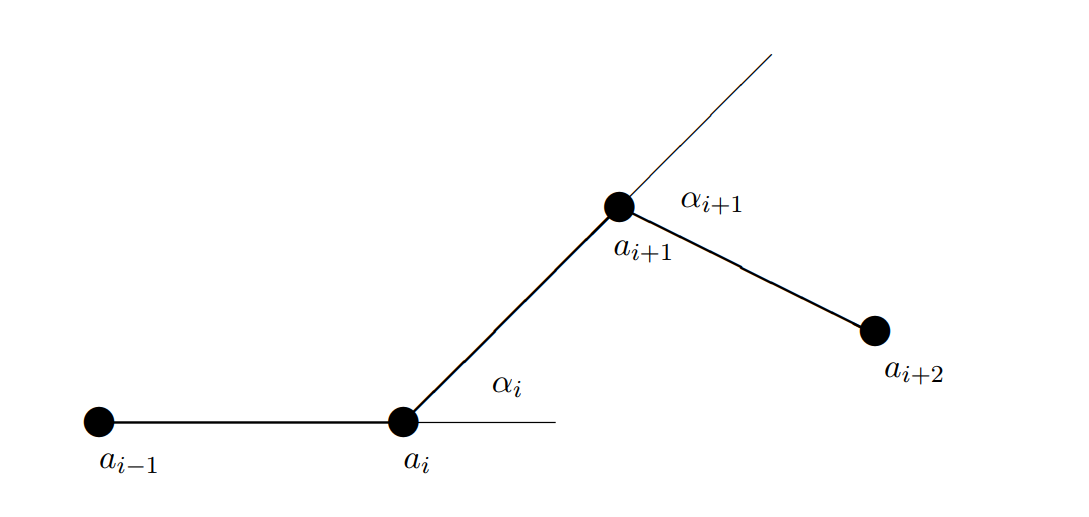
\includegraphics[scale=0.3]{configuration}
    \caption{Problem configuration}
    \label{atom configuration}
\end{figure}

There are several distinct advantages to this approach compared to using cartesian coordinates:
\begin{enumerate}
    \item Defining the bonded-molecule in terms of bond angles removes the need to recalculate the positions of atoms after a change (as the angles are relative).
    \item The cartesian coordinates can be obtained for any atom quickly via trigonometry.
    \item The vector of angles is a mathematically simpler representation of the problem and the change in energy for the cluster relative to the change in any angle can be determined.
\end{enumerate}
\par Representing chain molecules as 2-dimensional bonded molecules reduces the complexity of the model and also acts as a intermediary for developing algorithms that can optimize the configuration of molecules in 3 dimensions.

\section{Literature Review}
\subsection{BFGS}
\par The Broyden-Fletcher-Goldfarb-Shanno algorithm is an iterative method under the Quasi-Newton class of hill climbing algorithms. "Quasi-Newton methods, like steepest descent, require only the gradient of the objective function to be supplied at each iteration" \cite{numericalOptimization} 
\par Quasi-Newton methods are second order methods which use information about the derivative and second derivative of the function. BFGS is not an exact method as it approximates the Hessian using the differences in gradients over several iterations. The BFGS algorithm will never make a step in the `uphill' direction. To effectively make use of BFGS in problem spaces with local minima BFGS needs to be used as the local optimization step in a higher level global optimization algorithm such as a genetic population based search.

\subsection{Cross-Entropy Method}
The Cross-Entropy method is a generic approach to solving complicated optimization problems such as Max Cut or the travelling salesman problem. "the CE method... defines a precise mathematical frame-work for deriving fast, and in some sense "optimal" updating/learning rules..." \cite{CE}. The core algorithm of the CE method is quite a simple iterative process:
\begin{enumerate}
    \item Generate a sample of random data according to some mechanism.
    \item Score the sample and take an elite sub-sample of the resulting population.
    \item Use the values of the elite sub sample to update the parameters of the random mechanism to produce a "better" sample on the next iteration.
\end{enumerate}
\par The random mechanism can be as simple as specifying a parametric family of random distributions of the same length as the vector to be optimized (in this case the vector of angles) where the mean and standard deviation of each element in the parametric family are changed to reflect the elite sample after each generation. 
\par Specifying a smoothing parameter can be useful \cite{CE2}. The smoothing parameter determines the ratio of blending between the old and new distribution parameters. This smoothing parameter $\lambda$ can either be a static value $0 \leq \lambda \leq 1$ or dynamically changed as a function of time, score or another heuristic.

\section{Algorithm Description}
\subsection{Cross Entropy Optimization}
\subsubsection{Pseudocode}
\lstinputlisting[language=python]{Code/CE.py}

% \newpage
% \subsection{BFGS and Genetic Search}
% \subsubsection{Pseudocode}
% \lstinputlisting[language=python]{Code/BFGS.py}

\newpage
\subsection{Cross Entropy Method to Generate Optimization Candidates for BFGS}
\par An experiment to use the Cross Entropy Method as the global optimizer in order to generate optimization candidates for BFGS. Conceptually this method will allow the Cross Entropy Method to optimize the distribution vector to generate good candidates for BFGS optimization.
\begin{enumerate}
    \item Generate Population using distribution vector.
    \item Run BFGS on population members, generating an additional optimized population.
    \item Calculate the scores of the optimized population and sort.
    \item Update the distribution vector based on the pre-optimized sequences which correspond to the sequences in the elite sample of the optimized population.
    \item Goto step 1.
\end{enumerate}

The implementation of the algorithm is the same as the CE Method except the sequences generated are scored after a BFGS optimization step.

\section{Parameter Tuning}
\par The three configurable parameters for this implementation of the CE Method are:
\begin{itemize}[topsep=0pt]
    \item Population size
    \item Parameter blending
    \item Elite sample percentage
\end{itemize}
To examine the effects of changing each of the configurable parameters a base set of control parameters are chosen:
\begin{itemize}[topsep=0pt]
    \item Population size: 1000
    \item Parameter blending: 0.9
    \item Elite sample percentage: 0.1
\end{itemize}
The size of the molecule is set to N=40.

\subsection{Population Size}
\begin{figure}[H]
    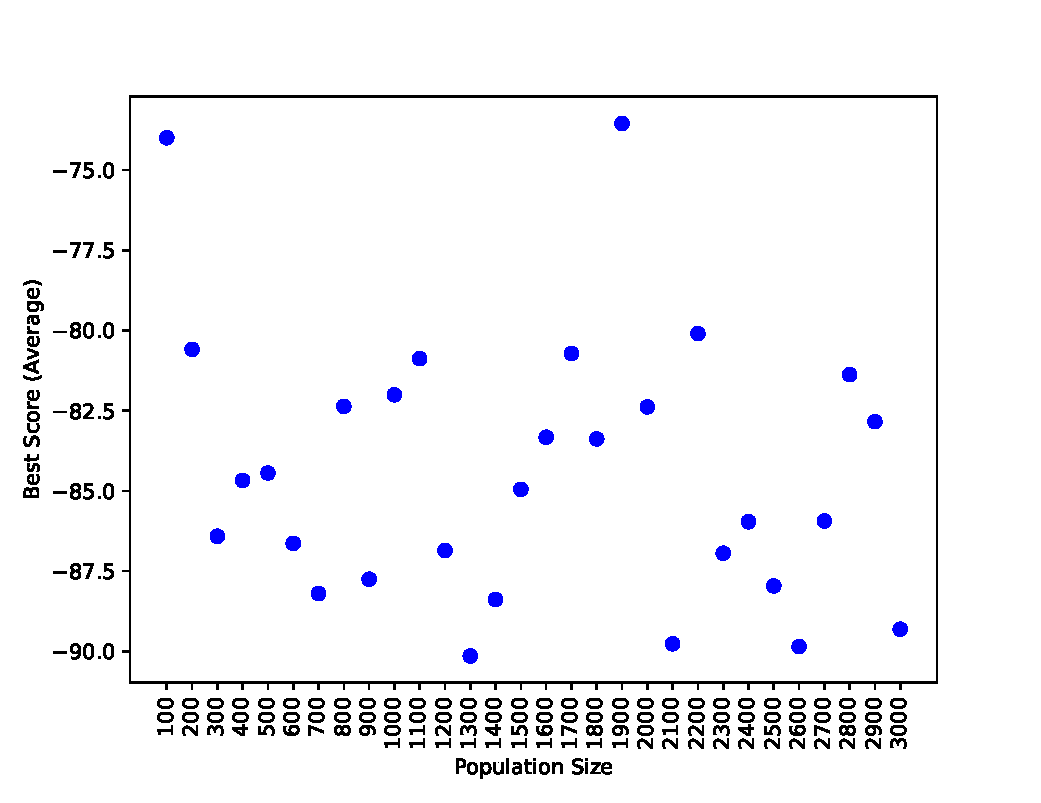
\includegraphics[scale=0.50]{CE_population}
    \caption{Population Size vs Score (Average over 3 runs)}
    \label{ce population}
\end{figure}
\par Figure \ref{ce population} shows how the change in population influences best score found by the optimizer. While there is no observable trend in the figure it is observed that population sizes below 300 result in very poor scores. The best scores are found in the range of 1300-3000 with no obvious determination as to which population values result in the best scores. Based on the data the optimal population size is determined to be 1300 as it is in the range of optimums and is not as computationally intensive as generating and processing larger populations.

\subsection{Elite Sample Size}
\begin{figure}[H]
    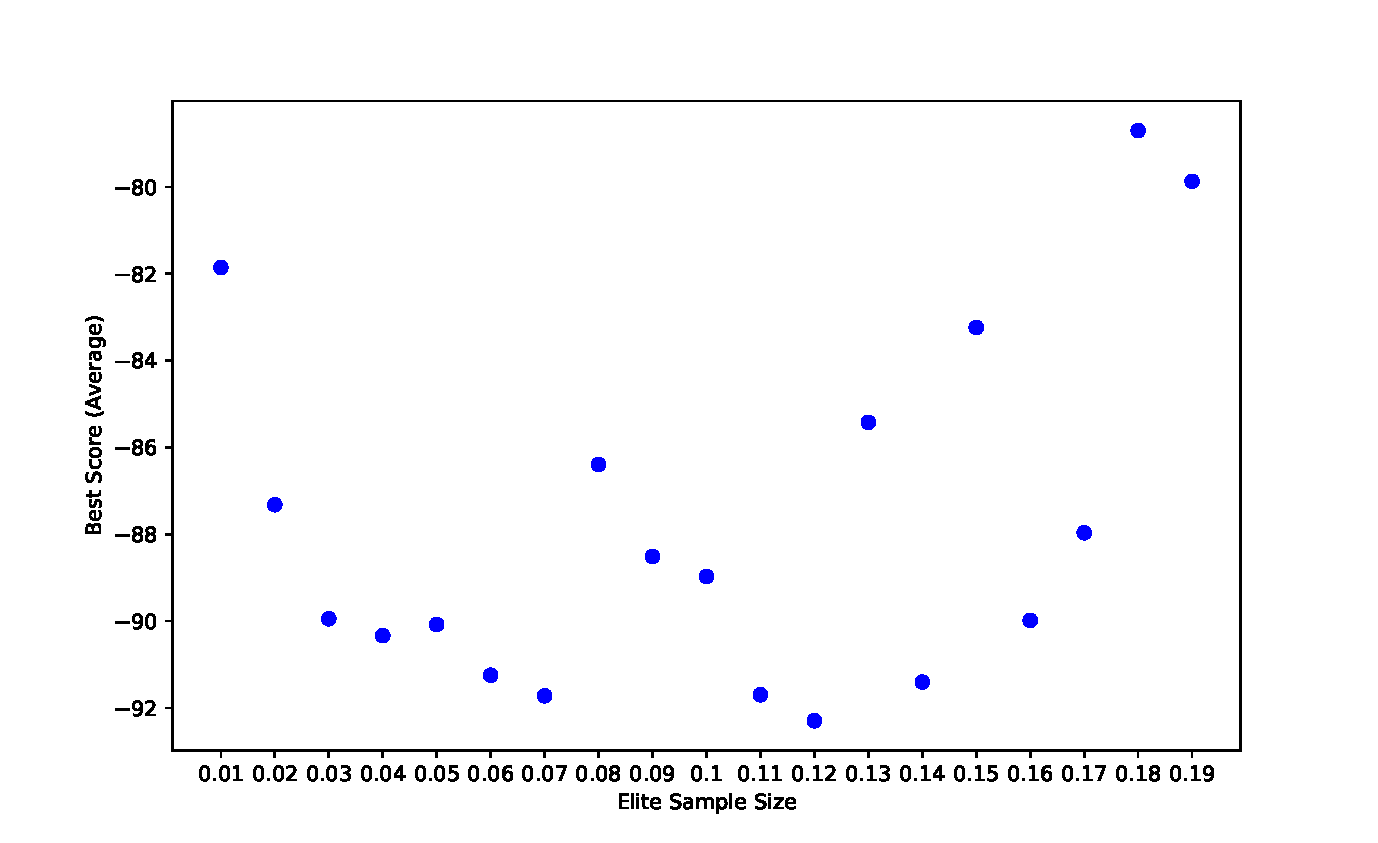
\includegraphics[scale=0.38]{CE_elitesample}
    \caption{Elite Sample \% vs Score (Average over 3 runs)}
    \label{ce elitesample}
\end{figure}

\par Figure \ref{ce elitesample} shows how the size of the elite sample influences the best scores found. It it clear from the graph that very small (5\% or less) and very large (15\% or greater) elite sample sizes have a detrimental effect to the effectiveness of the algorithm. The best scores clustering around the 11-12\% mark suggests that the ideal value for the size of the elite sample is 11-12\% of the population. Although if the size of the population is very large it may be advisable to reduce the size of the elite sample to increase selectivity. 

\subsection{Parameter Blending}
\begin{figure}[H]
    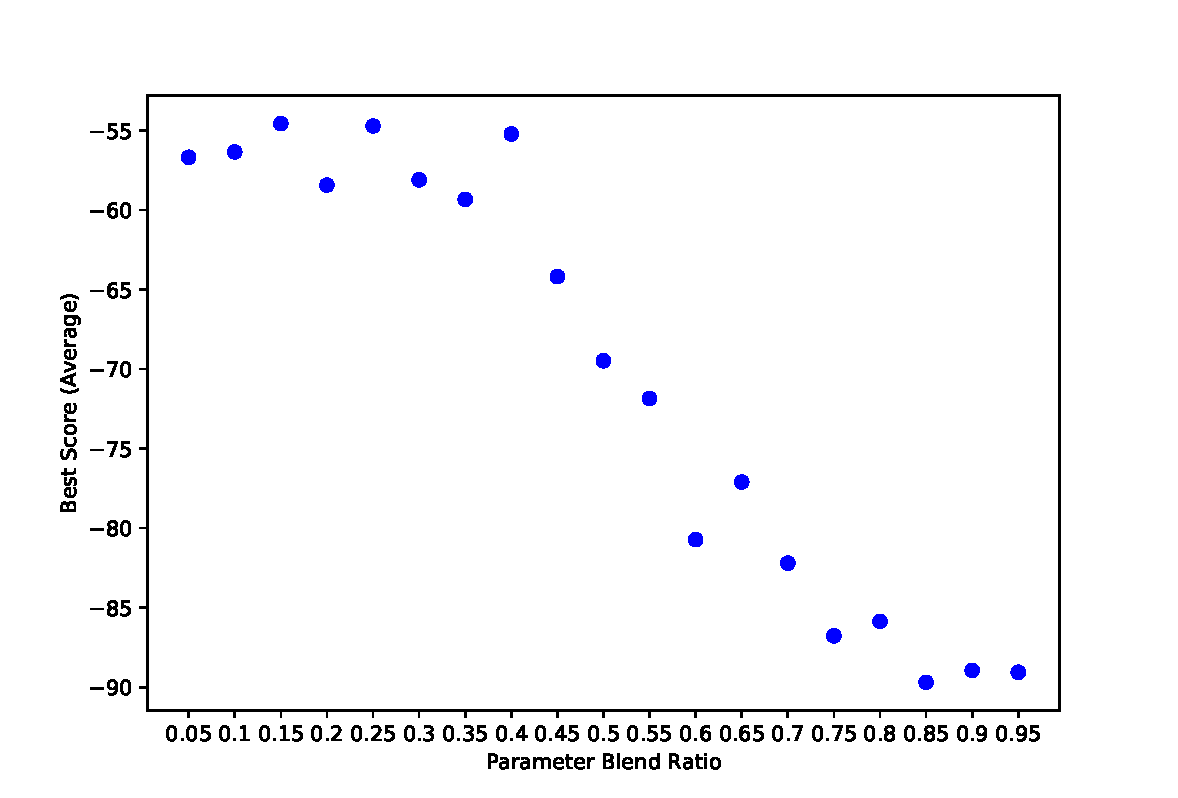
\includegraphics[scale=0.43]{CE_blending}
    \caption{Parameter Blending vs Score (Average over 3 runs)}
    \label{ce blending}
\end{figure}
\par Figure \ref{ce blending} shows a very clear downward trend which suggests that the ideal amount of parameter blending is minimal. Parameter blending in the range of 85-95\% gives the best results.

\subsection{Ideal Parameters - CE and BFGS}
\par After parameter optimization for the CE method the same parameters were used to achieve the best results when combining the CE Method with BFGS with the exception of population size. The BFGS optimization step is computationally intensive due to the calculation of energy gradients (see Appendix A) and the population size had to be decreased to 300 in order to speed up the algorithm and allow the global CE Optimizer to explore multiple minima without time constraint.

\section{Partial Restarting and Local Minima Hopping Methods}
\par As the CE Method will slowly converge on a local minima, different partial restart operators were tested in order to hop to other potentially better minima. Do detect the convergence to a local minima the algorithm compares the difference between the best score of the current population and the best score of the previous population. If this value becomes smaller than $\epsilon$ then the algorithm has converged and the optimizer will either return the result or partially reset. After convergence all generated members of the population with be representative of the distributions narrowed parameters (as the distribution's standard deviation parameter will narrow to near 0).

\subsection{Partial Random Reset}
After the algorithm reaches a certain $\epsilon$ each member of the parametric family has a certain percentage chance of being reset to the default distribution parameters.

\subsection{Partial Tail Reset}
After the algorithm reaches a certain $\epsilon$ a random number N is rolled and N distributions from the end of the parametric family are reset to default parameters.

\subsection{Gradient Ranked Partial Reset}
After the algorithm reaches a certain $\epsilon$ it calculates the gradient change in energy for each angle relative to the total energy of the cluster (see Appendix A). The gradients are then sorted by magnitude. The distributions corresponding to the greatest gradients are then reset in an attempt to introduce the most change in energy over subsequent generations while maintaining the general structure of the molecule.

\newpage
\section{Algorithm Performance}
\subsection{CE Method}
\begin{table}[!ht]
    \begin{tabularx}{\columnwidth}{XXXXXX}
    N  & Optimal & Best Found & N  & Optimal & Best Found \\ \hline
    4  & -5.1    & -5.07132   & 30 & -77.2   & -70.2578   \\
    5  & -7.2    & -7.15466   & 31 & -79.5   & -69.2296   \\
    6  & -9.3    & -9.29635   & 32 & -82.8   & -67.8379   \\
    7  & -12.5   & -12.427    & 33 & -86.1   & -75.3775   \\
    8  & -14.7   & -14.5394   & 34 & -88.3   & -77.1285   \\
    9  & -16.9   & -16.7548   & 35 & -91.7   & -81.6391   \\
    10 & -20.1   & -19.8421   & 36 & -95.0   & -82.3254   \\
    11 & -22.3   & -22.1631   & 37 & -98.3   & -89.7201   \\
    12 & -25.5   & -24.322    & 38 & -100.5  & -87.3879   \\
    13 & -27.8   & -27.5986   & 39 & -103.8  & -92.6629   \\
    14 & -31.0   & -29.7009   & 40 & -107.1  & -86.8567   \\
    15 & -33.2   & -32.8739   & 41 & -109.4  & -90.8365   \\
    16 & -36.5   & -33.1633   & 42 & -112.7  & -95.9652   \\
    17 & -38.7   & -35.2322   & 43 & -116.0  & -104.069   \\
    18 & -42.0   & -39.5358   & 44 & -119.3  & -102.404   \\
    19 & -45.3   & -42.1855   & 45 & -121.6  & -102.907   \\
    20 & -47.5   & -44.6016   & 46 & -124.9  & -104.417   \\
    21 & -50.8   & -47.1159   & 47 & -128.6  & -107.945   \\
    22 & -53.0   & -51.4069   & 48 & -131.5  & -109.423   \\
    23 & -56.3   & -48.5068   & 49 & -133.8  & -110.755   \\
    24 & -59.6   & -52.3969   & 50 & -137.1  & -114.764   \\
    25 & -61.8   & -53.2786   & 51 & -140.5  & -115.81    \\
    26 & -65.1   & -52.1118   & 52 & -143.7  & -116.132   \\
    27 & -68.4   & -61.5712   & 53 & -146.0  & -127.258   \\
    28 & -70.0   & -63.0996   & 54 & -149.3  & -124.026   \\
    29 & -74.0   & -64.3941   & 55 & -152.7  & -130.41    \\ \hline
    \end{tabularx}
    \caption{Best scores from Cross Entropy Method}
    \label{CE_Results}
\end{table}


\subsection{CE Method with BFGS}
\begin{table}[!ht]
    \begin{tabularx}{\columnwidth}{XXXXXX}
    N  & Optimal & Best Found & N  & Optimal & Best Found \\ \hline
    4  & -5.1    & -5.0717    & 30 & -77.2   & -64.042    \\
    5  & -7.2    & -7.16219   & 31 & -79.5   & -66.6319   \\
    6  & -9.3    & -9.34017   & 32 & -82.8   & -70.008    \\
    7  & -12.5   & -12.465    & 33 & -86.1   & -70.969    \\
    8  & -14.7   & -14.6329   & 34 & -88.3   & -72.8008   \\
    9  & -16.9   & -16.6597   & 35 & -91.7   & -78.7509   \\
    10 & -20.1   & -18.9354   & 36 & -95.0   & -77.1246   \\
    11 & -22.3   & -21.4258   & 37 & -98.3   & -80.0404   \\
    12 & -25.5   & -24.3834   & 38 & -100.5  & -79.7988   \\
    13 & -27.8   & -26.918    & 39 & -103.8  & -85.7043   \\
    14 & -31.0   & -29.6838   & 40 & -107.1  & -85.4764   \\
    15 & -33.2   & -32.6135   & 41 & -109.4  & -88.7995   \\
    16 & -36.5   & -33.9053   & 42 & -112.7  & -91.8655   \\
    17 & -38.7   & -36.9939   & 43 & -116.0  & -88.4889   \\
    18 & -42.0   & -38.1547   & 44 & -119.3  & -88.7862   \\
    19 & -45.3   & -41.6245   & 45 & -121.6  & -91.8972   \\
    20 & -47.5   & -44.8945   & 46 & -124.9  & -99.764    \\
    21 & -50.8   & -46.4786   & 47 & -128.6  & -98.9701   \\
    22 & -53.0   & -48.0152   & 48 & -131.5  & -102.948   \\
    23 & -56.3   & -51        & 49 & -133.8  & -97.7711   \\
    24 & -59.6   & -52.6622   & 50 & -137.1  & -103.551   \\
    25 & -61.8   & -54.948    & 51 & -140.5  & -105.572   \\
    26 & -65.1   & -57.8007   & 52 & -143.7  & -107.815   \\
    27 & -68.4   & -56.8625   & 53 & -146.0  & -106.928   \\
    28 & -70.0   & -60.2806   & 54 & -149.3  & -109.118   \\
    29 & -74.0   & -62.7181   & 55 & -152.7  & -118.146   \\ \hline
    \end{tabularx}
    \caption{Best scores from combination of BFGS and Cross Entropy Method}
    \label{BFGSCE_RESULTS}
\end{table}

\newpage
\section{Results}
The Cross Entropy Method was able to find near optimal values for values of N up to 20 and then configurations with scores within 5-15\% of the optimal values. The combination of the CE Method and BFGS yielded worse results do to the increased computational complexity and a lack of a strong driving force for global convergence.

\section{Conclusion}
Although the Cross Entropy Method (both as a local and global optimizer) was an ideal candidate to apply to the Bonded-Molecule problem the lack of ability to perform minima hopping in this implementation resulted in the algorithm not finding global minima for many lengths of molecules.

\clearpage
\bibliographystyle{apacite}
\bibliography{bib}

\clearpage

%
% ──────────────────────────────────────────────────────────── X ──────────
%   :::::: A P P E N D I C E S : :  :   :    :     :        :          :
% ──────────────────────────────────────────────────────────────────────
%
\appendices
\section{Gradient Calculation}
The total energy of the system is given by:
\begin{equation}
    V = \sum_{i<j}^{N}(\frac{1}{r_{ij}^{12}} - \frac{2}{r_{ij}^{6}})
\end{equation}
where
\begin{equation}
    r^{2}_{ij} = x^{2}_{ij} + y^{2}_{ij}
\end{equation}
Let
\begin{equation}
    \Psi_{k}=\sum_{i-1}^{k}\alpha_{i}
\end{equation}
and $(x_{0}, y_{0})=(0,0)$ and $\Psi_{0}=0$ then
\begin{equation}
    \begin{split}
        x_{i} = \sum_{k=0}^{i-1}\cos{\Psi_{k}} \\
        y_{i} = \sum_{k=0}^{i-1}\sin{\Psi_{k}}
    \end{split}
\end{equation}
Now
\begin{equation}
    V_{\alpha m} = \frac{-12 \sum_{i < j} (\frac{1}{r_{ij}^{13}} - \frac{1}{r_{ij}^{7}})}{r_{ij}}
\end{equation}
and
\begin{equation}
    (r_{ij})_{\alpha m} = \frac{((x_{i} - x_{j})(x_{i} - x_{j})_{\alpha m} + (y_{i} - y_{j})(y_{i} - y_{j})_{\alpha m}}{r_{ij}}
\end{equation}
assuming that $j > i$ we have
\begin{equation}
    \begin{split}
        (x_{i} - x_{j})_{\alpha m} = -\sum_{k=i}^{j-1}(\cos{\Psi_{k}})_{\alpha m} = \sum_{k=max(i,m)}^{j-1} \sin{\Psi_{k}} \\
        (y_{i} - y_{j})_{\alpha m} = -\sum_{k=i}^{j-1}(\sin{\Psi_{k}})_{\alpha m} = \sum_{k=max(i,m)}^{j-1} \cos{\Psi_{k}}
    \end{split}
\end{equation}
Therefore
\begin{equation}
    \begin{split}
        (r_{ij})_{\alpha m} = ((x_{i}-x_{j})(\sum_{k=max(i,m)}^{j-1}\sin{\Psi_{k}}) +\\
        (y_{i}-y_{j})(-\sum_{k=max(i, m)}^{j-1}\cos{\Psi_{k}}))/r_{ij}
    \end{split}
\end{equation}
which is zero when $m <= i$. Assuming $m > i$
\begin{equation}
    \begin{split}
        -\sum_{k=m}^{j-1}\cos{\Psi_{k}}=x_{j}-x_{m} \\
        -\sum_{k=m}^{j-1}\sin{\Psi_{k}}=y_{m}-y_{j}
    \end{split}
\end{equation}
and
\begin{equation}
    (r_{ij})_{\alpha m} = \frac{((x_{i} - x_{j})(y_{m} - y_{j}) + (y_{i} - y_{j})(x_{j} - x_{m})_{\alpha m}}{r_{ij}}
\end{equation}
Combining the terms we have
\begin{equation}
    \frac{\partial V}{\partial \alpha m} = -12 \sum_{i=0}^{m-1}\sum_{j=m+1}^{n}(\frac{1}{r_{ij}^{14}} - \frac{1}{r_{ij}^{8}})((x_{i}-x_{j})(y_{m}-y_{i})+(y_{i}-y_{j})(x_{j}-x_{m}))
\end{equation}

%
% ─── END ────────────────────────────────────────────────────────────────────────
%
\end{document}
